%!TEX root = graduate-work.tex
% Добавьте ссылку на файлы с текстом работы
% Можно использовать команды:
%   \input или \include
% Пример:
%    \input{mainfiles/1-section} или \include{mainfiles/2-section}
% Команда \input позволяет включить текст файла без дополнительной обработки
% Команда \include при включении файла добавляет до него и после него команду
% перехода на новую страницу. Кроме того, она позволяет компилировать каждый файл
% в отдельности, что ускоряет сборку проекта.
% ВАЖНО: команда \include не поддерживает включение файлов, в которых уже содержится команда \include,
% т.е. не возможен рекурсивный вызов \include
\newcommand*{\Source}{
    %!TEX root = ../graduate-work.tex
\phantomsection
\section*{Введение} 
\addcontentsline{toc}{section}{Введение}
Криптосистема Мак-Элиса "--- одна из старейших криптосистем с открытым ключом. Она была предложена в 1978
Р.~Дж.~Мак-Элисом~\cite{MCEliece}. Данная криптосистема
основывается на $\mathbf{\mathbb {NP}}$-трудной проблеме в теории
кодирования. Основная идея её построения  состоит в маскировке
некоторого кода, имеющего эффективные алгоритмы декодирования, под
код, не обладающий видимой алгебраической и комбинаторной
структурой, такие коды принято называть кодами общего положения.
Эта криптосистема обладает одним важным преимуществом "--- высокой
скоростью зашифрования и расшифрования. Однако, у неё имеется
серьёзный недостаток "--- относительно низкая скорость передачи
($R$). Обычно у кодовых криптосистем $R<1$, тогда как у
криптосистемы RSA скорость в точности равна $1$.

В этой работе рассматривается обобщение криптосистемы
Мак-Элиса, предложенное в 1994 коду В.М.
Сидельниковым~\cite{Sidelnikov1}. В этой работе модификация,
предложенная В.~М.~Сидельниковым, называется криптосистемой\\
Мак-Элиса--Сидельникова. Криптосистема Мак-Элиса--Сидельникова
строится на основе $u$-кратного использования кодов Рида--Маллера
$RM(r,m)$. Она имеет высокую криптографическую стойкость, скорость
передачи близкую к $1$ и сравнительно невысокую сложность
шифрования секретных сообщений и расшифрования криптограмм этих
сообщений.

В работе исследуются вопросы, связанные с пространством
эквивалентных секретных ключей, то есть секретных ключей,
порождающих одинаковые открытые ключи, новой криптосистемы. Опишем
краткое содержание разделов работы.

В \S~1 даётся определение криптосистемы Мак-Элиса, описываются её
секретный и открытый ключи. Приводятся алгоритмы зашифрования и
расшифрования.

В \S~2 изучается ключевое пространство криптосистемы Мак-Элиса.
Устанавливается связь классов эквивалентностей секретных ключей с
группой автоморфизмов линейного кода, лежащего в основе этой
криптосистемы.

В \S~3 описывается криптосистема Мак-Элиса--Сидельникова:
секретный и открытый ключи, алгоритмы зашифрования и
расшифрования.

\S~4 посвящён ключевому пространству новой криптосистемы. В нём
вводятся множества, необходимые для описания классов
эквивалентности секретных ключей. Получаются нижние и верхние
оценки на мощности  введённых множеств и на число открытых ключей
криптосистемы Мак-Элиса--Сидельникова.

В \S~5 изучается криптосистема Мак-Элиса--Сидельникова в случае
двух блоков ($u=2$).

В настоящей работе получаются нижние оценки на мощность множества
открытых ключей криптосистемы
Мак-Элиса--Сидельникова(теорема~\ref{t3}) при использовании
произвольного числа блоков $u$. Для кодов Рида--Маллера с
$u$-кратным повторением строится множество, которое, в некотором
смысле, является аналогом группы автоморфизмов обычного кода
Рида--Маллера, и устанавливается связь этого множества с классами
эквивалентности секретных ключей.

Для случая двух блоков ($u=2$) полностью описывается указанное
множество при использовании кодов Рида--Маллера $RM(r,m)$
$(r\leqslant 2,r<m)$ и матриц определённого вида
(теоремы~\ref{theorem1},~\ref{theorem2}). Тем самым при $u=2,
r\geqslant 2, r<m$ описываются все классы эквивалентности
секретных ключей с представителями особого вида и вычисляются их
мощности. Для некоторых классов эквивалентности секретных ключей
приводятся нижние оценки на их мощность(теоремы~\ref{theorem1}
и~\ref{theorem2}).

    %!TEX root = ../graduate-work.tex

\section{Историческая справка}

\subsection{История возникновения}

Интегрирование как операция восходит к античной математике, где её использовали
для нахождения площадей, объёмов и других величин. Уже в трудах Архимеда можно
встретить методы, похожие на интегрирование, но в более примитивной форме. В
эпоху Возрождения и в XVII-XVIII веках математики начали формализовать понятие
интеграла. Особенно важным был вклад Исаака Ньютона и Готфрида Лейбница,
которые независимо друг от друга разработали основы дифференциального и
интегрального исчисления.

Тем не менее, проблема точного и формального определения интеграла оставалась
актуальной. До XIX века существовали разные подходы к нахождению площадей и
объёмов, но их формулировки не имели строгой математической основы.

\subsection{Идея Римана}

В середине XIX века Бернард Риман предложил новую концепцию интеграла, которая
стала общепринятой в математике. Его идея заключалась в следующем: для
вычисления интеграла функции, заданной на отрезке
$[a, b]$, нужно разбиение этого отрезка на небольшие части (сегменты), на
которых функция приближенно представляется простыми величинами
(например, прямыми отрезками или прямоугольниками).

Риман предложил делить отрезок $[a, b]$ на $n$ частей, вычислять сумму
произведений высоты функции на ширину каждого интервала, а затем исследовать
поведение этой суммы, когда разбиение становится всё более тонким. Если такая
сумма сходится к определённому значению при бесконечно мелком разбиении, то
говорят, что функция интегрируема в смысле Римана.

\subsection{Развитие и расширения}

Позднее, на рубеже XIX-XX веков, математики начали развивать и обобщать понятие
интеграла. Одним из значительных шагов стало введение обобщённых понятий
интегралов, таких как интеграл Лебега, который позволяет интегрировать более
широкие классы функций, включая те, которые не являются интегрируемыми
по Риману. Эти обобщения стали важными для теории вероятностей и других
областей математики.

Тем не менее, интеграл Римана остаётся важным инструментом для понимания
основной идеи интеграции и продолжает использоваться во многих областях,
включая физику, инженерию и экономику.


    %!TEX root = ../graduate-work.tex

\section{Определение и свойства интеграла Римана}

\subsection{Классическое определение}

Пусть дана функция \( f(x) \), определённая на отрезке \( [a, b] \), где \(a <
b\). Разбиение отрезка \( [a, b] \) на \( n \) частей будет состоять из
последовательности точек \( a = x_0 < x_1 < \dots < x_n = b \), которая делит
интервал \( [a, b] \) на подынтервалы \( [x_{i-1}, x_i] \), где \( i = 1, 2,
\dots, n \). Каждый подынтервал имеет длину \( \Delta x_i = x_i - x_{i-1} \).

Для каждого подынтервала выбирается произвольная точка \( x_i^* \), в которой
функция \( f(x) \) оценивается. Сумма Римана для функции \( f(x) \) относительно
разбиения \( P = \{ x_0, x_1, \dots, x_n \} \) и точек \( x_i^* \) на каждом
подынтервале записывается как:

\[ S(f, P) = \sum_{i=1}^{n} f(x_i^*) \Delta x_i.  \]

Интеграл Римана функции \( f(x) \) на отрезке \( [a, b] \) определяется как
предел этой суммы, когда максимальная длина интервала \( \|P\| \) стремится к
нулю, то есть:

\[ \int_a^b f(x) \, dx = \lim_{\|P\| \to 0} S(f, P), \]

где \( \|P\| \) — максимальная длина подынтервала в разбиении \( P \).

Если этот предел существует, то функция \( f(x) \) называется интегрируемой в
смысле Римана на отрезке \( [a, b] \), и её интеграл на данном интервале
существует.

\begin{figure}[h]
\center{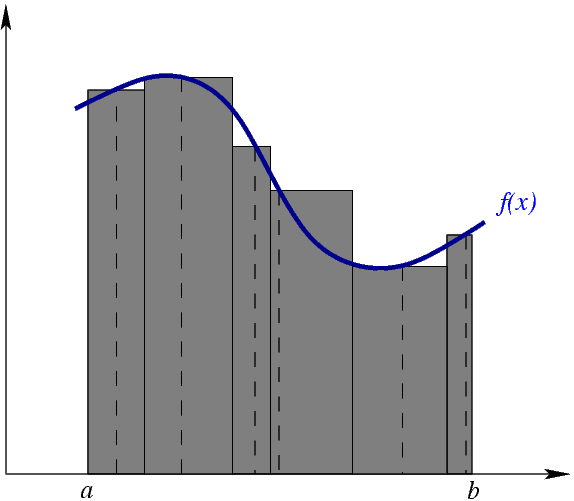
\includegraphics[width=1\linewidth]{integral}}
\caption{Геометрический смысл интеграла Римана }
\end{figure}

\subsection{Общие соображения об условиях интегрируемости}

Для того чтобы функция \( f(x) \) была интегрируемой в смысле Римана на отрезке
\( [a, b] \), она должна удовлетворять некоторым условиям. Во-первых, функция \(
f(x) \) должна быть ограниченной на отрезке \( [a, b] \). Во-вторых, она не
должна иметь слишком много разрывов. Точное требование состоит в том, что \(
f(x) \) должна быть ограниченной и иметь конечное число разрывов на
рассматриваемом интервале.

Пример функции, не интегрируемой по Риману, — это функция Дирихле на интервале
\( [0, 1] \), которая принимает значение 1 для рациональных чисел \( x \) и 0
для иррациональных чисел. Эта функция имеет бесконечно много разрывов, и её
интеграл по Риману не существует.

\subsection{Свойства интеграла Римана}

Интеграл Римана обладает рядом важных свойств, которые делают его удобным
инструментом для анализа функций. Рассмотрим несколько из них.

\subsubsection{Линейность}

Интеграл Римана обладает свойством линейности. Если \( f(x) \) и \( g(x) \) —
интегрируемые функции на отрезке \( [a, b] \), то линейная комбинация этих
функций также будет интегрируемой, причём интеграл линейной комбинации равен
линейной комбинации интегралов:

\[ \int_a^b \left( c_1 f(x) + c_2 g(x) \right) \, dx = c_1 \int_a^b f(x) \, dx +
c_2 \int_a^b g(x) \, dx, \]

где \( c_1 \) и \( c_2 \) — произвольные константы.

\subsubsection{Аддитивность}

Интеграл Римана обладает свойством аддитивности. Если отрезок \( [a, b] \)
разбить на два подынтервала \( [a, c] \) и \( [c, b] \), то интеграл на всём
интервале \( [a, b] \) равен сумме интегралов на этих подынтервалах:

\[ \int_a^b f(x) \, dx = \int_a^c f(x) \, dx + \int_c^b f(x) \, dx.  \]

Это свойство позволяет вычислять интеграл функции на сложном интервале, разбив
его на более простые части.

\subsubsection{Монотонность}

Если функция \( f(x) \) меньше или равна функции \( g(x) \) на всём интервале \(
[a, b] \), то интеграл функции \( f(x) \) меньше или равен интегралу функции \(
g(x) \):

\[ \int_a^b f(x) \, dx \leq \int_a^b g(x) \, dx.  \]

Это свойство является полезным при сравнении интегралов различных функций.

\subsubsection{Интегрируемость композиции}

Если функция \( f(x) \) интегрируема на отрезке \( [a, b] \), а функция \( g(x)
\) непрерывна на этом отрезке, то композиция \( f(g(x)) \) также будет
интегрируемой на \( [a, b] \).

\subsubsection{Интеграл и предел}

Если функция \( f(x) \) интегрируема на \( [a, b] \), а последовательность
функций \( \{ f_n(x) \} \) сходится к функции \( f(x) \) почти всюду на
интервале \( [a, b] \), то при условии, что последовательность \( \{ f_n(x) \}
\) ограничена, верно:

\[ \lim_{n \to \infty} \int_a^b f_n(x) \, dx = \int_a^b \lim_{n \to \infty}
f_n(x) \, dx = \int_a^b f(x) \, dx.  \]

Это свойство известно как теорема о пределе интегралов и является важным
инструментом для анализа предельных процессов.

    %!TEX root = ../graduate-work.tex

\section{Верхние и нижние суммы интеграла Римана}

Для того чтобы строго определить класс интегрируемых функций в смысле Римана, используем
верхние и нижние суммы.

\begin{figure}[h]
	\center{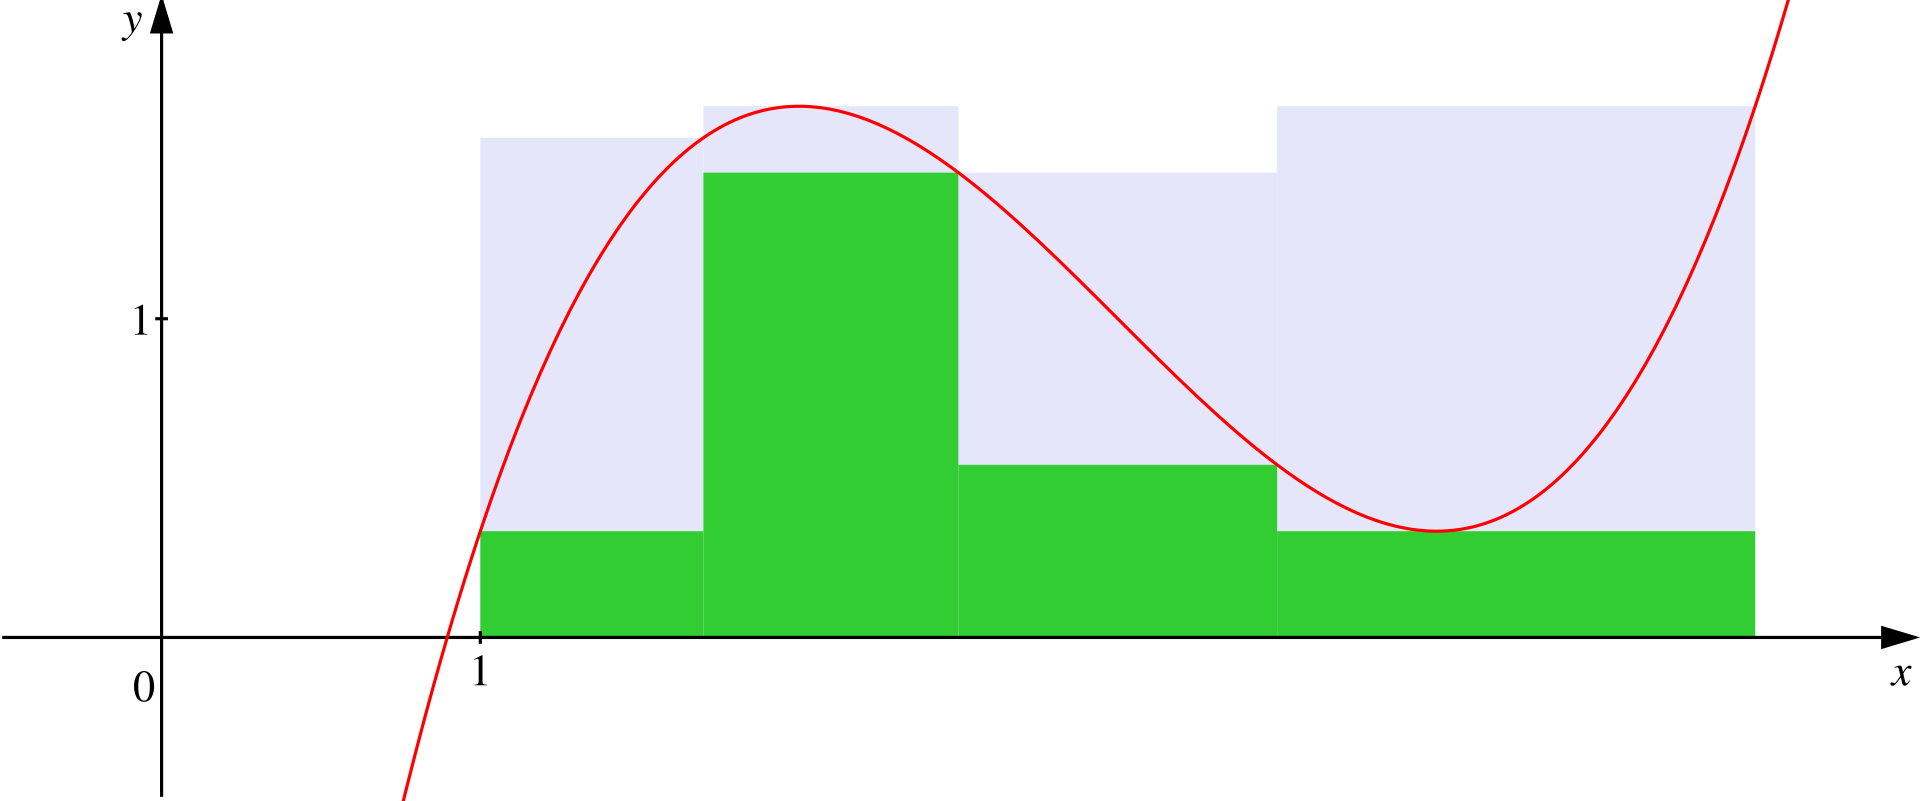
\includegraphics[width=1\linewidth]{upperlower}}
	\caption{Нижняя (зеленая) и верхняя (серая) суммы Дарбу на 4 отрезках разбиения}
	%\label{ris:image}
\end{figure}

\subsection*{Разбиение интервала}

Пусть дана функция \( f(x) \), определённая на отрезке \( [a, b] \). Разбиение
интервала \( [a, b] \) состоит из последовательности точек \( a = x_0 < x_1 <
\dots < x_n = b \), которое делит этот интервал на \( n \) подынтервалов:

\[ \Delta x_i = x_i - x_{i-1}, \quad i = 1, 2, \dots, n.  \]

Каждому подынтервалу \( [x_{i-1}, x_i] \) соответствует несколько значений
функции \( f(x) \) в его пределах.

\subsection{Нижняя сумма Римана}

Нижняя сумма Римана \( L(P, f) \) для разбиения \( P = \{x_0, x_1, \dots, x_n\}
\) и функции \( f(x) \) определяется как сумма произведений длины каждого
подынтервала на инфимум функции \( f(x) \) на этом подынтервале. То есть для
каждого \( i \)-го подынтервала \( [x_{i-1}, x_i] \) выбирается точка, в
которой функция \( f(x) \) принимает минимальное значение:

\[ L(P, f) = \sum_{i=1}^{n} \inf_{x \in [x_{i-1}, x_i]} f(x) \Delta x_i.  \]

Интуитивно, нижняя сумма Римана представляет собой сумму площадей
прямоугольников, где высоты прямоугольников определяются минимальными
значениями функции на каждом подынтервале.

\subsection{Верхняя сумма Римана}

Верхняя сумма Римана \( U(P, f) \) для разбиения \( P \) и функции \( f(x) \)
определяется как сумма произведений длины каждого подынтервала на супремум
функции \( f(x) \) на этом подынтервале. То есть для каждого \( i \)-го
подынтервала \( [x_{i-1}, x_i] \) выбирается точка, в которой функция \( f(x)
\) принимает максимальное значение:

\[ U(P, f) = \sum_{i=1}^{n} \sup_{x \in [x_{i-1}, x_i]} f(x) \Delta x_i.  \]

Таким образом, верхняя сумма Римана представляет собой сумму площадей
прямоугольников, где высоты прямоугольников определяются максимальными
значениями функции на каждом подынтервале.

\subsection{Основное свойство верхних и нижних сумм}

Верхняя и нижняя суммы \( U(P, f) \) и \( L(P, f) \) всегда удовлетворяют
неравенству:

\[ L(P, f) \leq \int_a^b f(x) \, dx \leq U(P, f), \]

где \( \int_a^b f(x) \, dx \) — это значение интеграла Римана, если оно
существует. Таким образом, нижняя и верхняя суммы дают <<ограничения>> на
значение интеграла, и если эти суммы сходятся друг к другу при бесконечно
тонком разбиении, то интеграл Римана существует.

\section{Класс интегрируемых по Риману функций}

Интеграл Римана применяется только к определённому классу функций, которые
называются интегрируемыми по Риману. Эти функции обладают рядом характеристик,
которые позволяют корректно вычислить их интегралы на отрезке \( [a, b] \). В
данной главе рассматриваются основные свойства и критерии для функций,
интегрируемых по Риману.


\subsection{Условия интегрируемости по Риману}

Для того чтобы функция \( f(x) \) была интегрируемой по Риману на отрезке \(
[a, b] \), она должна удовлетворять следующим основным условиям:

\begin{itemize} \item \textbf{Ограниченность.} Функция \( f(x) \) должна быть
			ограниченной на интервале \( [a, b] \). То есть, существует
			такая константа \( M \), что для всех \( x \in [a, b] \)
			выполняется неравенство \( |f(x)| \leq M \).
    
		\item \textbf{Наличие конечного числа разрывов.} Функция \( f(x) \)
			может иметь на интервале \( [a, b] \) разрывы, однако их должно
			быть конечное количество. Если функция имеет бесконечно много
			разрывов, то её интеграл по Риману не существует. Это означает,
			что функция должна быть непрерывной, за исключением конечного
числа разрывов.  \end{itemize}

Примером функции, не интегрируемой по Риману, является функция Дирихле на
интервале \( [0, 1] \), которая принимает значение 1 для рациональных чисел \(
x \) и 0 для иррациональных чисел. Эта функция имеет несчётное число разрывов
на интервале, и её интеграл не существует.

\subsection{Классы интегрируемых функций}

Класс интегрируемых по Риману функций включает в себя множество типов функций,
среди которых выделяются:

\begin{itemize} \item \textbf{Непрерывные функции.} Все функции, которые
			непрерывны на отрезке \( [a, b] \), интегрируемы по Риману. Это
			связано с тем, что непрерывность функции на замкнутом отрезке
			гарантирует, что функция ограничена и не имеет разрывов.
    
		\item \textbf{Функции с конечным числом разрывов.} Функции, имеющие
			конечное количество разрывов на отрезке \( [a, b] \), также
			являются интегрируемыми по Риману. Важно, что эти разрывы не
			могут быть "слишком большими" (например, функции с бесконечными
			разрывами или с бесконечно большим скачком значений не
			интегрируемы).
    
		\item \textbf{Простейшие полиномы и рациональные функции.} Полиномы и
			рациональные функции, ограниченные на интервале, всегда
			интегрируемы по Риману, так как они непрерывны на данном
			интервале.
    
		\item \textbf{Монотонные функции.} Монотонные функции на отрезке \(
			[a, b] \) всегда интегрируемы по Риману, поскольку они
			ограничены и имеют не более конечного числа разрывов.
\end{itemize}

\subsection{Критерий с использованием верхних и нижних сумм}

Функция \( f(x) \) интегрируема по Риману на интервале \( [a, b] \), если и
только если для любого \( \epsilon > 0 \) существует такое разбиение \( P \),
что разница между верхней и нижней суммами будет меньше \( \epsilon \), то
есть:

\[ U(P, f) - L(P, f) < \epsilon.  \]

Это условие гарантирует, что функция можно аппроксимировать с точностью до \(
\epsilon \) с помощью верхних и нижних сумм, и, следовательно, существует
интеграл Римана функции на данном интервале.

\section{Заключение}

Интеграл Римана сыграл ключевую роль в развитии математического анализа,
предоставив чёткую формализацию вычисления площадей, объёмов и других величин.
Его введение стало важной вехой в истории математики, и несмотря на
существование обобщений, интеграл Римана остаётся
одним из основополагающих понятий в математическом анализе. Его применение
охватывает множество областей математики, физики и инженерии.






}


% Информация о годе выполнения работы
\def\Year{%
    % 2006%
    \the\year%     % Текущий год
}

% Укажите тип работы
% Например:
%     Выпускная квалификационная работа,
%     Магистерская диссертация,
%     Курсовая работа, реферат и т.п.
\def\WorkType{%
    % Выпускная квалификационная работа%
    % Магистерская диссертация%
    Курсовая работа%
    % Реферат%
    % Дипломная работа%
}

% Название работы
%%%%%%%%%%% ВНИМАНИЕ! %%%%%%%%%%%%%%%%
% В МГУ ОНО ДОЛЖНО В ТОЧНОСТИ
% СООТВЕТСТВОВАТЬ ВЫПИСКЕ ИЗ ПРИКАЗА
% УТОЧНИТЕ НАЗВАНИЕ В УЧЕБНОЙ ЧАСТИ
\def\Title{%
    Интеграл Римана%
}


% Имя автора работы
\def\Author{%
    Заботин Михаил Алексеевич%
}

% Информация о научном руководителе
%% Фамилия Имя Отчество%
\def\SciAdvisor{%
    Чупраков Дмитрий Вячеславович%
}
%% В формате: И.~О.~Фамилия%
\def\SciAdvisorShort{%
    Д.~В.~Чупраков%
}
%% должность научного руководителя
\def\Position{%
    % профессор%
    доцент%
    % старший преподаватель%
    % преподаватель%
    % ассистент%
    % ведущий научный сотрудник%
    % старший научный сотрудник%
    % научный сотрудник%
    % младший научный сотрудник%
}
%% учёная степень научного руководителя
\def\AcademicDegree{%
    % д.ф.-м.н.%
    % д.т.н.%
    к.ф.-м.н.%
    % к.т.н.%
    % без степени%
}

% Информация об организации, в которой выполнена работа
%% Город
\def\Place{%
    Киров%
}
%% Университет
\def\Univer{%
    Вятский государственный университет%
}
%% Факультет
\def\Faculty{%
    Факультет компьютерных и физико-математических наук%
}
%% Кафедра    
\def\Department{%
    Кафедра фундаментальной математики%
}     

%%%% Переключите статус документа для отладки
%%%% В режиме draft документ собирается очень быстро
%%%% и выводится полезная информация о том
%%%% какие строки вылезают за границы документа, что удобно для борьбы с ними
\def\Status{%
    % draft%
    final%
}

%%%% Включает и выключает подпись <<С текстом работы ознакомлен>>
\def\EnableSign{%
    % true%
}
